\chapter{Fejlesztői dokumentáció}
\label{ch:impl}

\textbf{TODO: intro}

\section{Csomagok}

A szoftver forráskódja több csomagban és modulban található.
A forrráskód jelentős része öt fő csomagba van szerveze,
ezek az alábbi táblázatban láthatók.

\begin{table}[H]
	\centering
	\begin{tabular}{ | m{0.25\textwidth} | m{0.65\textwidth} | }
		\hline
		\textbf{Csomag} & \textbf{Rövid leírás} \\
		\hline \hline
		\emph{app} & GUI alkalmazás csomagja \\
		\hline
		\emph{client} & adatbázis kliens \\
		\hline
		\emph{model} & adatok modelezése és mentése \\
		\hline
		\emph{tests} & egység és egyéb tesztek \\
		\hline
		\emph{transformations} & átalakítások forráskódja és API az átalakításokhoz \\
		\hline
	\end{tabular}
	\caption{A szoftver fő csomagjai}
	\label{tab:packages}
\end{table}

Minden csomag a szoftver egy jól elkülöníthető részét vagy funkcióját valósítja meg.
A fő csomagok (a \emph{tests} csomag kivételével) nem tartalmaznak "futtatható" fájlokat,
a belépési pontok külön modulokba vannak szervezve.

\section{\emph{app} csomag}

Az \emph{app} csomag feladata az átalakításokat szemléltető GUI-s alkalmazás megvalósítása.
Az alkalmazás architektúrája model-nézet-kontroller (MVC) szerű.
Egy nézet rendelkezik egy kontrollerrel és a kontroller pedig egy modellel.

A nézet feladata a GUI definiálása és frissítése,
a model feladata az adatelérés vagy az alkalmazás állapotának modelezése.
A kontroller ezt a két réteget köti össze,
így a nézet nem függ a modeltől és a model sem a nézettől.

Tegyük fel, hogy a nézeten történik egy GUI esemény, például a felhasználó egy gombra klikkel,
aminek az eseménykezelője a model használatát igényli.
Ekkor az eseménykezelő a nézet kontrollerének továbbítja a megfelelő adatokat.
A kontroller használja a modelt, majd a nézetet direk vagy indirekt módon frissíti.
Direkt módon frissíti, ha a modeltől kapott adatokat a nézetnek továbbítja,
ha pedig egy eseményt vált ki a modelben aminek hatására a nézet frissül akkor indirekt frissíti.
Ezt a működést az alábbi ábrán láthatjuk.

\begin{figure}[H]
	\centering
	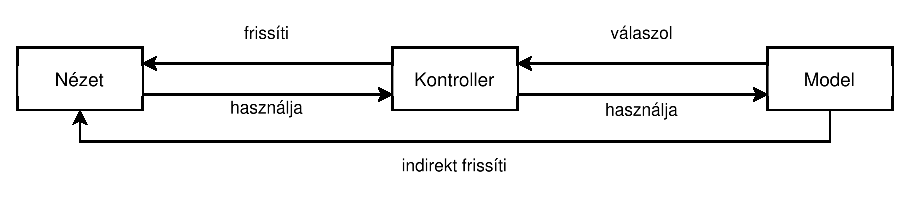
\includegraphics[width=0.9\textwidth]{images/figs/mvc.eps}
	\caption{Egy esemény kezelése az MVC architektúrában}
\end{figure}

\subsection{Állapotmodel}

Az alkalmazásban kétféle model különböztethető meg: az állapot és adatelérési modelek.
Az alkalmazás állapotmodelje az \emph{app.appstate} modulban található.
Az adatelérési modelek nem az alkalmazás csomagjában vannak definiálva mivel 
a szoftver más rétegeinek is szüksége van ezekre.

Az állapotmodel az \emph{observer} tervezési mintát használja a nézetek frissítésére
és az \emph{AppState} osztályban van definiálva.
Az \emph{AppState} osztály az \emph{Observable} osztályból származik,
ezért rendelkezik megfigyelők (\emph{observers}) egy listájával,
ami esemény-eseménykezelő párok listája.

Ha a nézet egy komponenesét az állapotmodel változásának hatására akarjuk frissíteni,
akkor azt az eseménykezelőt, ami frissíti, hozzárendelhetjük az állapotmodel egy eseményéhez.

Hozzárendelni egy eseménykezelőt egy eseményhez az \emph{Observable} osztály \emph{attach}
metódusával lehet.
Ha az adott eseményt kiváltja egy változás a modelben, akkor a model értesíti a nézeteket,
vagyis az \emph{observers}-ben az eseményéhez rendelt eseménykezelőket meghívja,
a frissítéshez szükséges adatokat paraméterként továbbítva.

\begin{figure}[H]
	\centering
	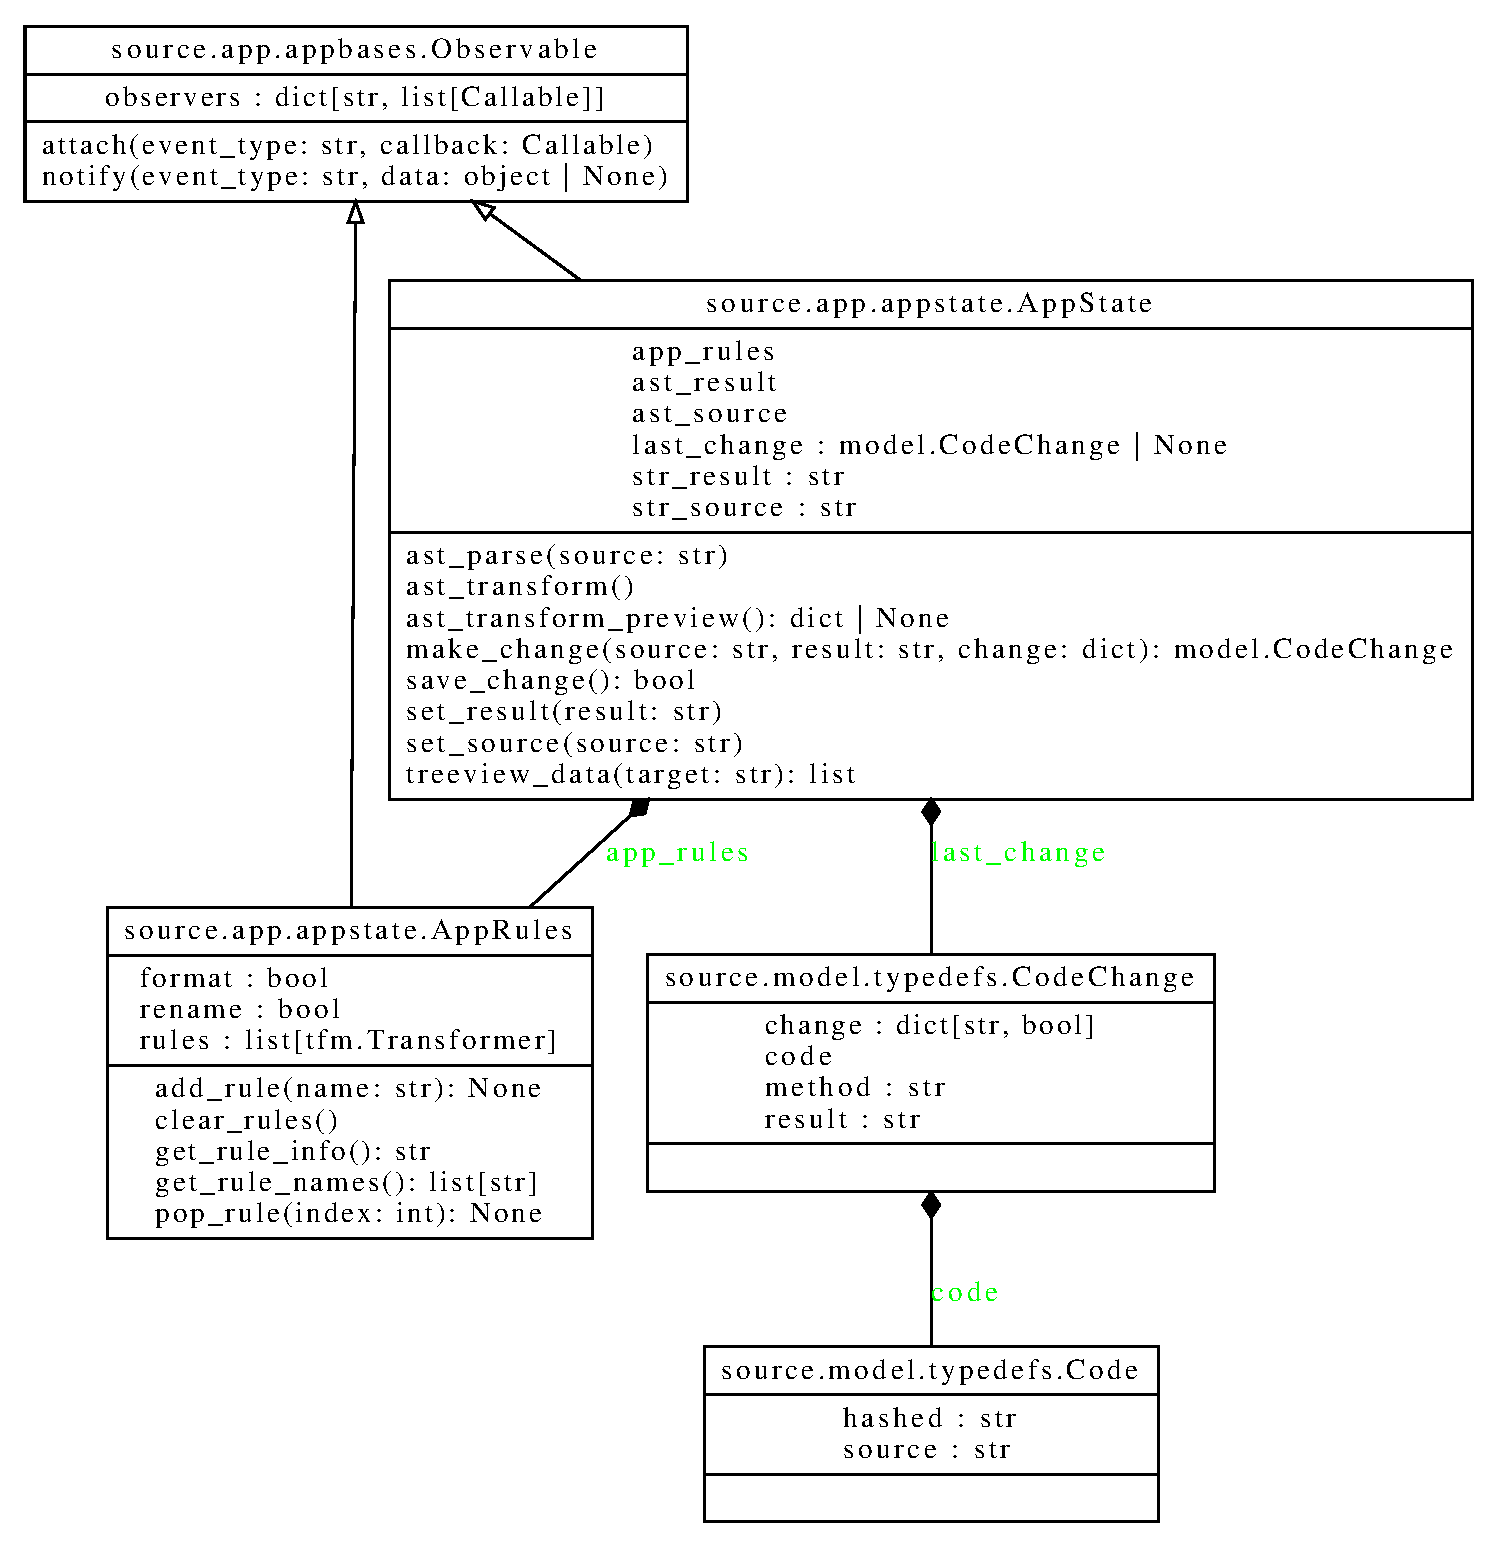
\includegraphics[width=0.9\textwidth]{images/uml/AppState.eps}
	\caption{Állapotmodel UML diagramja}
\end{figure}

\pagebreak

A felhasználói felület (View-réteg) kódja a \emph{app.views} csomagban található,
a Python-ban alapból megtalálható \emph{tkinter} könyvtárt használja, amit az 
erre építő \emph{ttkbootstrap} könyvtárral egészít ki.

A kontrollerek feladata a kommunikáció a modelek és nézetek között.
Csak a felhasználói felület két fő nézete
a \emph{RefactorTab} és a \emph{DatabaseTab} 
rendelkeznek saját kontrollerekkel.